Pour valider notre modèle, nous avons développé une simulation basée sur un graphe.
Chaque machine de notre système y est représentée par un nœud, et possède en moyenne \textit{l} liaisons vers d'autres machines

\begin{figure}[ht]
\centering
     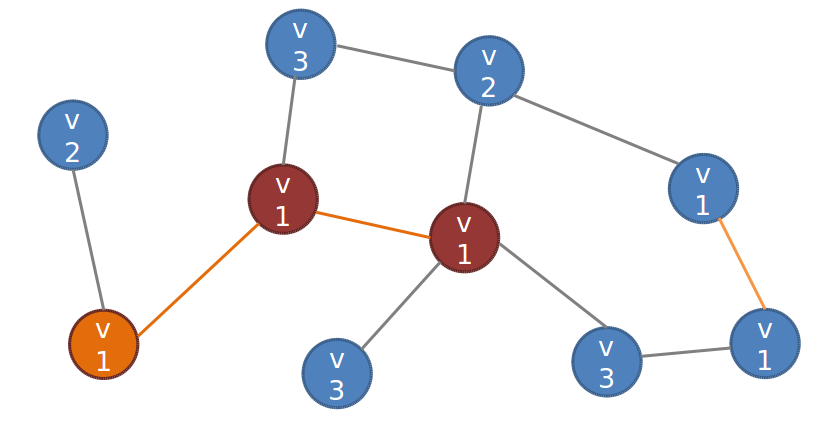
\includegraphics[width=1.0\linewidth]{Paul/python/graph.png}
     \caption{Représentation du système par un graphe}
     \label{normal_case}
\end{figure}

La première étape est de définir la répartition des versions dans le système. Afin de faire varier l'entropie, on utilise une distribution de Dirichlet.

\begin{figure}[ht]
\centering
     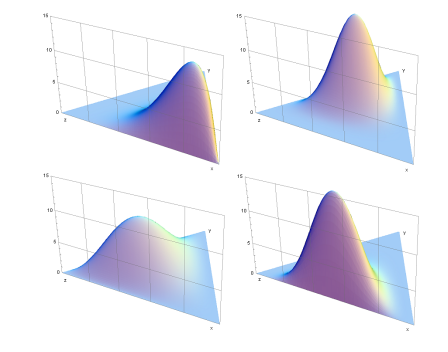
\includegraphics[width=1.0\linewidth]{Paul/dirichlet.png}
     \caption{Distribution de Dirichlet (source: Wikipedia)}
     \label{normal_case}
\end{figure}
